\documentclass[conference]{IEEEtran}
\IEEEoverridecommandlockouts
%\documentclass[a4paper,12pt]{article}

%vorgegeben
\usepackage{balance}
\usepackage{graphicx}
\usepackage{booktabs}
\usepackage{relsize}
\usepackage{pgfplots}
\usepackage{tabularx}
\usepackage{gensymb}
\usepackage{caption}
\usepackage{listings}
\usepackage{babel}
\usepackage{siunitx}
\usepackage{url}
\usepackage{subcaption}
\usepackage{comment}
\usepackage{tikz}

%packages to eneble new font
\usepackage{fontspec}
\setmainfont{Myriad Pro}
%\setsansfont{Myriad Pro}
%\newfontfamily\computermodern{Computer Modern}
%\setsansfont{Latin Modern}

%no Idea why I have these
\usepackage[utf8]{inputenc}
\usepackage{amsmath}
\usepackage{hyperref}

%to enble captions vor the graphics
\usepackage{caption}

\usepackage{array} %enebels tabular

%neue pacages vom neuen Template
\usepackage{cite}
\usepackage{amssymb,amsfonts} %hier vorher: \usepackage{amsmath,amssymb,amsfonts}
\usepackage{algorithmic}
\usepackage{textcomp}
\usepackage{xcolor}
\usepackage{epstopdf}
\usepackage{multirow}
\usepackage{blindtext}
\pgfplotsset{compat=1.18}
\title{\textbf{Short Paper:} IoT-NDN: An IoT Architecture via Named Data
Netwoking (NDN)\\}
\author{Leonard Boetefuer}
\date{\today}


\begin{document}

\maketitle

\begin{abstract}
  The Internet of Things (IoT) is gaining importance in everyday life, science, and industry. 
  While current IoT systems can be modeled in IP, 
  future systems with over a billion devices will face great challenges. 
  Data aggregation, naming scalability, 
  and the handling of resource-restrained devices are problems that need to be solved. 
  Named Data Networking (NDN), addresses many issues by using named data. 
  IoT based on NDN (IoT-NDN) is to solve many issues that are mentioned in this work.
  
  \end{abstract}
  
  \section{Introduction}
  
  
  
  This short paper is based on \cite{b99}.
  %The Internet of Things (IoT) is gaining importance in everyday life, science, and industry.
  % warum IP schlecht ist
  Currently, the Internet Protocol (IP) is used in IoT, but it lacks scalability, robustness, and efficiency. Mobility isn't supported in the location-based IP; protocols are needed for support.
  %warum NDN cool ist
  Named Data Network (NDN) is data and not location-focused; it allows devices to request data using unique, location-independent names. NDN offers scalability, lightweight configuration, and simplified communications, resulting in NDN being a solution for IoT systems \cite{b1}.
  
   
  %\section{Related Work}
  %XYZTEST2
  %braucht man das???? wahrscheinlich nicht
  \section{Analysis of IoT and NDN}
  This section will discuss the limitations of IoT devices and the challenges of the current Internet architecture.
  \subsection{Challanges of the IoT}
  1) \textbf{The connectivity of IoT devices:}
  Currently, IoT devices use a server-client or host-to-host connection, neither is scalable enough for a billion devices.
  %The server-client architecture has a bottleneck in the server.
  %was für ein Bottlenck (nur ein server kann durch anfragen überlastet werden)
  In the host-host architecture, every host has to communicate with every other host, resulting in exponential resource consumption.
  %The server-client and the host-to-host model both need IP addresses for every single device, which is not possible with a billion devices.
  %NDN solves the IP shortage and it is de-central helps with the bottleneck
  %100
  
  2) \textbf{Technological Standards:}
  The current standards are inadequate for network protocols, communication protocols, and data aggregation. They lead to inefficient caching and aggregation. 
  In addition, mobility protocols are needed to mitigate the effect of a connection loss. 
  %vielleicht schöner und/oder kürzer
  %97
  
  3) \textbf{Mobility:}
  IoT systems that use mobile devices need to note, that devices are numerous and technologically diverse, and consumer reliance is increasing. 
  % über 90
  
  
  4) \textbf{Complexity and Integration Issues:}
  IoT systems comprise many unique Application Programming Interfaces (APIs), protocols, and platforms. 
  %APIs expeccially are not desined with the resource limitations of IoT devices in mind. 
  % maybe add that later
  The integration of technologies into the system is very complicated due to all the different combinations. This system should consider the resource limitation of its components.
  %100
  
  \subsection{NDN for the IoT}
  %erstes mal NDN erwähnt (auser intorduction)
  
  1) \textbf{NDN Packet Length:}
  Packages in NDN are not bound to a specific length, which allows expansion of further protocols by adding or subtracting from the overhead.
  IoT devices are limited in memory, resulting in small packages with a necessity of a small overhead.
  %100
  
  
  
  %Packages in NDN are not bound to a specific length. This is helpful to expand further protocols by adding or subtracting from the overhead.
  %IoT devices will send only small packages; because of the limited resources in memory, resulting in the necessity of a small overhead.
  
  %The overhead must be kept small because the information proportion of small packets is much more influenced by a large overhead.
  %to many packages will drain energy and put strain on the network.
  %Quelle 16 (nicht benutzt)
  2) \textbf{Caching in IoT/NDN:}
  IoT devices have too little memory for efficient caching, resulting in higher unnecessary package flow and a reduction in data availability.
  The solution is in-network caching, a feature of NDN.  
  % wie wird in-network caching grob umgesetzt?
  
  %ALTER TEXT
  %Data freshness and reduced unnecessary package flow, is achieved by integrating an in-network cache, which is a feature of NDN.
  %To keep the data up to date and reduce unnecessary package flow, we need to integrate caches into the system. 
  %The problem is that the small devices don't have enough memory to keep an efficient cache. 
  %The solution is to use in-network caching, a feature of NDN.
  %ganz kurz in-network caching erklären.
  %Quelle 11
  %Even a small cache will dramatically increase the data availability [11].
  %Quelle 2
  
  
  3) \textbf{Data Aggregation in Wireless Networks:}
  If a user requests data that includes multiple packages, each package will be requested separately (excluding the others). This results in a greater overhead and more unnecessary package flow. The new system should fix the request problem.
  %93
  
  4) \textbf{Naming Problems in Wireless Networks:}
  NDN supports name-centric services, which facilitates access without knowing their location. There is still a need to automate naming conventions, because of the size of the networks. These names should be kept short to minimize storage usage \cite{b17}\cite{b18}. 
  %Quelle 18 (3 mal)
  
  
  5) \textbf{Routing Scalability in NDN:}
  In NDN routing is managed by names, instead of usual number based systems. The scalability of routing is important to facilitate a large network.
  % Da fehlt was mach das vielleicht später
  % Quelle 19 und 20
  
  \section{Architecture of IoT-NDN System}
  
  %die Tabelle muss an die richtige stelle.
  \begin{figure}[h]
      \centering
      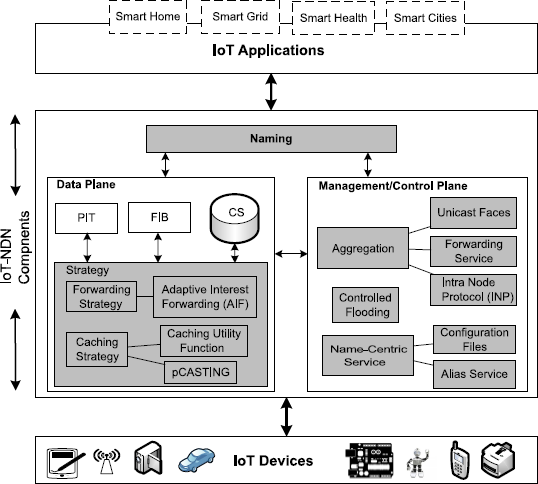
\includegraphics[width=0.25\textwidth]{IoT-NDN_System_architecture_and_its_components.png}\\
      \caption{IoT-NDN System architecture and its components}
      \label{fig:enter-label}
  \end{figure}
  
  The IoT-NDN has three main components that are responsible for packages, caching, strategies, 
  and others.
  % The \textbf{naming} component is made up of naming schemes and a structure for wireless networks.
  % The \textbf{Management and control plane} is made up of Unicast Faces, Forwarding Services Intra Node Protocol, Controlled Flooding, Configuration, and Alias services. %aus Paper Zitiert. Vielleicht über graphic kürzen.
  % The \textbf{dataplan} component is made up of the caching and forwarding strategies. 
   %grey component?
  
  %Was ist CS, PIT und FIB? Wofür stehen die Abkürzungen?
  
  Devices in the IoT-NDN architecture have three tables: CS, PIT and FIB.
  %Quelle 2
  % NDN solves many issues discussed in II. For more information, refer to Tabel 1.
  
  %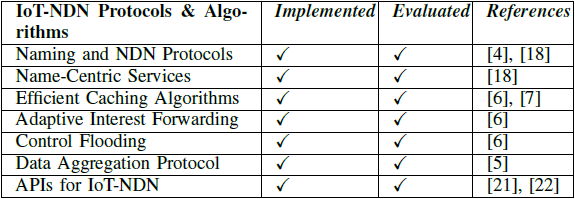
\includegraphics[width=0.3\textwidth]{IMPLEMENTED_AND_TESTED_PROTOCOLS_AND_ALGORITHMS_IN_IOT-NDN.png}\\
  
  
  % {\tiny
  % \begin{table}[h]
  % \caption{Implemented and tested Protocols and Algorithms in IoT-NDN}
  % \begin{tabular}{ | m{2,6cm} | m{1,5cm}| m{1,5cm} |  m{1,5cm} |} 
  
  %   \hline
  %   \textbf{IoT-NDN Protocols \& Algorithms}& \textbf{Implemented} & \textbf{Evaluation} & \textbf{References} \\ 
  %   \hline
  %   Naming and NDN Protocols & \checkmark & \checkmark & \cite{b4},\cite{b18} \\ 
  %   \hline
  %   Name-Centric Services & \checkmark & \checkmark & \cite{b18}\\ 
  %   \hline
  %   Efficient Caching Algorithm & \checkmark & \checkmark & \cite{b6},\cite{b7} \\ 
  %   \hline
  %   Adaptive Internet Forwarding & \checkmark & \checkmark & \cite{b6} \\ 
  %   \hline
  %   Control Flooding & \checkmark & \checkmark & \cite{b6} \\ 
  %   \hline
  %   Data Aggregation Protocol & \checkmark & \checkmark & \cite{b5} \\ 
  %   \hline
  %   APIs for IoT-NDN & \checkmark & \checkmark & \cite{b21},\cite{b22} \\ 
  %   \hline
  
  % \end{tabular}
  % \end{table}
  % }
  
  \subsection{Naming}
  %muss an die richtige stelle (unter naming)
  \begin{figure}[h]
      \centering
      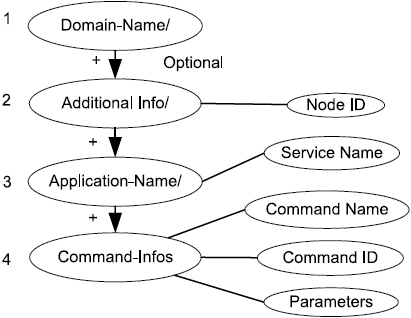
\includegraphics[width=0.25\textwidth]{Name_Structure_of_the_suggested_Approach.png}\\
      \caption{Name Structure of the suggested Approach}
      \label{fig:enter-label}
  \end{figure}
  
  In IoT-NDN the structure in which data is addressed is hierarchical, as shown in Fig. 2.
  The first component is a global domain name. 
  % The second is optional and, if used, stores additional information, like the node ID.
  % The third component contains the application and service name.
  % The fourth component contains the command name, command ID, and additional parameters.
  The marker component is the additional fifth component of the name, specific to IoT-NDN.
  It contains application, service, or device resource information.
  %was kann sie und wofür braucht man sie?
  
  \subsection{Managment and Control Plane}
  %wenn zeit Enumeration????
  %ich kann 5 umsonst zitieren
  1) \textbf{Aggregation:} Combining similar information into one package will reduce the memory stress and energy consumption of the Content Store (CS) \cite{b5}.
  Data aggregation is achieved by three components. The components are: Forwarding Service, Unicast Faces, and Intra Node Protocol (INP). They are explained in greater detail in \cite{b5}.
  
  %erkläre Unicast Faces.#
  %was ist radio layer (die sicherungsschicht?)
  Unicast Face needs every package (in the radio layer) to include the source and destination address. 
  When a device receives a package, it will build a connection to the sender of the package. 
  %This enables devices to learn their neighbors. 
  If a connection is lost, for this connection allocated resources will be released. 
  %später noch ergänzen
  
  2) \textbf{Controlled Flooding:}
  
  %überarbeiet muss nochmal überarbeiet werden
  IoT devices aren't reliable in power or connectivity, usually resulting in the Forwarding Information Base (FIB) tables not being populated in advance by routing information. Controlled flooding is used for its robustness and by adding a timer-based package suppression, overhead can be reduced. Packages won't be sent out while the timer is running, if the same package is received it will only be sent out once.
  
  %muss ich 13 und 23 zitieren?
  %IoT devices aren't reliable in power or connectivity. % 70%sicher
  %As a result, the Forwarding Information Base (FIB) tables won't usually be populated in advance by routing information. %ziemlich eins zu eins übernommen
  %Packages will transfer from one device to another and to mitigate flooding, controlled flooding is used.
  %To reduce overhead and redundancy, devices will delay sending out packages. This time can be random or based on network topology.
  %While a package is delayed and arrives  again at the same device, the package is not send out twice. 
  %The path is selected
  %MUSS NOCH PATH SELECTION MACHEN
  
  3) \textbf{Name-Centric Services:}
  The use of a gateway enables IoT-Devices to be reachable from any internet device. 
  The gateway allows wireless and wired connections, via protocol conversion. 
  It provides all important configurations of names and  IoT-NDN devices. Services on the gateway can be developed as IoT-NDN applications, enabling communication to each other threw the IoT-NDN daemon and face. 
  In order to reduce the workload on the IoT devices the gateway will use aliases (that are shorter) to reduce the size of the packages.
  Names received from the internet will be mapped to names used in the Iot-NDN network.
  
  \subsection{Data Plane}
  1) \textbf{Strategy-In-Network Caching:} 
  The CS is a caching place in IoT-NDN devices, unlike routers in the Internet Protocol it can send cached packages more than once.
  If a device receives a package request, it will first check the CS by checking for matching prefixes. 
  This is done because the same data will probably be requested many times in IoT-NDN networks.
  The standard replacement strategy is LRU, but others can be implemented. %LFU und randome auch gut mit quelle 7 und 26
  IoT-NDN devices have a special probabilistic CAching STrategy (pCASTING), that considers data freshness and the charge and storage of devices. This strategy is used %among other things
  when a device receives a data package with a matching PIT.
  % vieleicht mehr über pCasting, dann aber auch quelle 7 zitiern
  
  2) \textbf{Strategy-Forwarding:}
  The forwarding path is selected from the FIB to forward Interest packets, by the forwarding strategy component. 
  By remembering the number of unsatisfied interests, the forwarding strategy could be used to control the traffic.
  The forwarding component is the path of the interest by using data such as delay and throughput. 
  Forwarding steps on devices are supported by IoT-NDN and the forwarding strategy allows the request of lost packages in network, by using its metrics. 
  These metrics can be used to study the performance of every face.
  Finding missing packages can also be achieved with the InterestLifeTime parameter. For more information, see \cite{b6}
  
  \section{Conclusion}
  First, the paper highlights the problems of IoT if implemented in IP. 
  %Then it examines cache mechanisms, data aggregation and naming in wireless networks.
  NDN isn't built with resource-constrained devices in mind. This paper names the problems and solutions to integrate NDN into IoT.
  The result Iot-NDN is a new type of network that includes communication and data access, based on names.
  %97
  
  \begin{thebibliography}{00}
  \bibitem{b99}M. A. Heil, "IoT-NDN: An IoT Architecture via Named Data
  Netwoking (NDN)" "in" Software Embedded System Department
  Euroimmun AG, a PerkinElmer Company
  \bibitem{b1} Z. Sheng, S. Yang, Y. Yu, A. V. Vasilakos, J. A. Mccann, and K. K.
  Leung, “A survey on the ietf protocol suite for the internet of things:
  standards, challenges, and opportunities,” IEEE Wireless Communications,
  vol. 20, no. 6, pp. 91–98, December 2013.
  % \bibitem{b4} Z. Ren, M. Hail, and H. Hellbruck, “Ccn-wsn - a lightweight, flexible
  % content-centric networking protocol for wireless sensor networks,” in
  % Intelligent Sensors, Sensor Networks and Information Processing, 2013.
  \bibitem{b5} T. Teubler, M. A. M. Hail, and H. Hellbr¨uck, “Efficient Data Aggregation
  with CCNx in Wireless Sensor Networks,” in 19th EUNICE Workshop
  on Advances in Communication Networking (EUNICE 2013), Germany.
  \bibitem{b6}M. A. Hail, M. Amadeo, A. Molinaro, and S. Fischer, “On the performance
  of caching and forwarding in information centric networking for
  the iot,” in 13th International Conference on Wired and Wireless Internet
  % Communications, April 2015.
  % \bibitem{b7}——, “Caching in named data networking for the wireless internet
  % of things,” in Recent Advances in Internet of Things (RIoT), 2015
  % International Conference on, April 2015, pp. 1–6.
  \bibitem{b17}V. Jacobson, D. K. Smetters, J. D. Thornton, M. F. Plass, N. H. Briggs,
  and R. L. Braynard, “Networking named content,” in Proceedings of the
  5th International Conference on Emerging Networking Experiments and
  Technologies, ser. CoNEXT ’09. New York, NY, USA: ACM, 2009, pp.
  1–12. [Online]. Available: http://doi.acm.org/10.1145/1658939.1658941
  \bibitem{b18}T. Teubler, M. A. M. Hail, and H. Hellbr¨uck, “A solution for the
  naming problem for name-centric services,” in Wired/Wireless Internet
  Communications, A. Mellouk, S. Fowler, S. Hoceini, and B. Daachi,
  Eds. Cham: Springer International Publishing, 2014, pp. 214–227.
  % \bibitem{b21}S. Ebers, M. A. Hail, S. Fischer, and H. Hellbr¨uck, “Api for data
  % dissemination protocols - evaluation with autocast,” in The Third World
  % Congress on Nature and Biologically Inspired Computing (NaBIC 2011).
  % Salamanca, Spain: IEEE, Oct. 2011, pp. 534–539.
  % \bibitem{b22}M. A. Hail and S. Fischer, “Flexible API for IoT Services with Named
  % Data Networking,” in 2016 IEEE International Conference on Emerging
  % Technologies and Innovative Business Practices for the Transformation
  % of Societies (IEEE EmergiTech 2016), Mauritius, Mauritius, Aug 2016.
  \end{thebibliography}
  \end{document}